% !TeX program = xelatex
\documentclass[a4paper,14pt,oneside,openany]{memoir}

%%% Поля, отступы, интервал %%%
\usepackage[left=30mm, right=15mm, top=20mm, bottom=20mm]{geometry}
\pagestyle{plain}
\parindent=1.25cm
\usepackage{indentfirst}
\OnehalfSpacing
\raggedbottom % Не растягивать вертикально

%%% Язык и шрифты (XeLaTeX) %%%
\usepackage{polyglossia}
\setdefaultlanguage[indentfirst=true,forceheadingpunctuation=false]{russian}
\setotherlanguages{english}
\setmainfont{FreeSerif}
\setsansfont{FreeSans}
\setmonofont{FreeMono}

%%% Доп. типографика против вылезания текста %%%
\usepackage{microtype}
\usepackage{xurl}
\urlstyle{same}
\usepackage[htt]{hyphenat} % переносы в \texttt
\sloppy % Более свободная вёрстка

%%% Переносы %%%
\tolerance=1200
\hbadness=2000
\emergencystretch=3em
\hfuzz=0.5pt
\vfuzz=\hfuzz
\clubpenalty=10000
\widowpenalty=10000
\brokenpenalty=4991

%%% Кириллица для списков %%%
\makeatletter
\def\russian@Alph#1{\ifcase#1\or
  А\or Б\or В\or Г\or Д\or Е\or Ж\or
  И\or К\or Л\or М\or Н\or
  П\or Р\or С\or Т\or У\or Ф\or Х\or
  Ц\or Ш\or Щ\or Э\or Ю\or Я\else\xpg@ill@value{#1}{russian@Alph}\fi}
\def\russian@alph#1{\ifcase#1\or
  а\or б\or в\or г\or д\or е\or ж\or
  и\or к\or л\or м\or н\or
  п\or р\or с\or т\or у\or ф\or х\or
  ц\or ш\or щ\or э\or ю\or я\else\xpg@ill@value{#1}{russian@alph}\fi}
\makeatother

%%% Рисунки, таблицы, подписи %%%
\usepackage{graphicx,caption,subcaption,float}
\graphicspath{{images/}}
\captionsetup[figure]{font=small,width=\textwidth,name=Рисунок,justification=centering}
% \captionsetup[subfigure]{font=small} % Закомментировано - не используется
\captionsetup[table]{singlelinecheck=false,font=small,width=\textwidth,justification=justified}
\captiondelim{ --- }
\setkeys{Gin}{width=\textwidth}
\renewcommand{\thesubfigure}{\asbuk{subfigure}}
\usepackage[section]{placeins}

%%% Гиперссылки %%%
\usepackage{hyperref}
\hypersetup{
    colorlinks=true,
    linktoc=all,
    linktocpage=true,
    linkcolor=red,
    citecolor=red
}

%%% Списки %%%
\usepackage{enumitem}
\renewcommand*{\labelitemi}{\normalfont{--}}
\makeatletter
\AddEnumerateCounter{\asbuk}{\russian@alph}
\makeatother
\renewcommand{\labelenumii}{\asbuk{enumii})}
\renewcommand{\labelenumiii}{\arabic{enumiii})}
\setlist{noitemsep, leftmargin=*}
\setlist[1]{labelindent=\parindent}
\setlist[2]{leftmargin=\parindent}
\setlist[3]{leftmargin=\parindent}

%%% Нумерация %%%
\counterwithout{figure}{chapter}
\counterwithout{equation}{chapter}
\counterwithout{table}{chapter}

%%% Библиография (ГОСТ) %%%
\usepackage{csquotes}
\usepackage[backend=biber,style=gost-numeric,sorting=none]{biblatex}
\addbibresource{bibl.bib}

%%% Дополнительные пакеты %%%
\usepackage{longtable,ltcaption}
\usepackage{multirow,makecell}
\usepackage{booktabs}
\usepackage{soul} % ИСПРАВЛЕНО: soul вместо soulutf8
\usepackage{icomma}
\usepackage{hyphenat}
\usepackage{textcomp}
\usepackage[version=4]{mhchem}
\usepackage{amsmath,amssymb}
\usepackage{etoolbox}

%%% Листинги кода (с запретом разрывов) %%%
\usepackage{listings}
\usepackage{xcolor}
\lstset{
    basicstyle=\small\ttfamily,
    keywordstyle=\color{blue!70!black}\bfseries,
    commentstyle=\color{gray!70},
    stringstyle=\color{orange!80!black},
    breaklines=true,
    breakatwhitespace=false,
    columns=fullflexible,
    keepspaces=true,
    frame=single,
    numbers=left,
    numberstyle=\tiny\color{gray},
    showstringspaces=false,
    tabsize=4,
    captionpos=b,
    xleftmargin=0.5em,
    xrightmargin=0pt,
    breakautoindent=true,
    aboveskip=10pt,
    belowskip=10pt
}

% Запрет разрыва lstlisting между страницами
\BeforeBeginEnvironment{lstlisting}{\begin{samepage}}
\AfterEndEnvironment{lstlisting}{\end{samepage}\vspace{2pt}}

\lstdefinelanguage{Kotlin}{
    keywords={fun,val,var,class,data,object,if,else,when,for,while,
              return,import,package,is,as,in,out,override,private,public,
              companion,init,null,true,false,this,super,interface,abstract,
              open,by,sealed,suspend,runBlocking,launch,async},
    morecomment=[l]{//},
    morecomment=[s]{/*}{*/},
    morestring=[b]"
}
\lstdefinelanguage{CppSeventeen}{
    morekeywords={int,double,float,char,bool,void,auto,const,static,struct,
                  class,public,private,protected,namespace,using,new,delete,
                  true,false,nullptr,std,string,vector,map,unordered_map,
                  thread,mutex,atomic,function,lock_guard,unique_lock,
                  shared_ptr,make_shared,this,return,if,else,for,while,do,
                  switch,case,break,continue,default,try,catch,throw,noexcept,
                  decltype,sizeof,alignof,alignas,constexpr,enum,typedef,
                  inline,extern,volatile},
    morecomment=[l]{//},
    morecomment=[s]{/*}{*/},
    morestring=[b]",
    sensitive=true
}

%%% TikZ для схем %%%
\usepackage{tikz}
\usetikzlibrary{arrows.meta,positioning,fit,calc,shapes.geometric}
\tikzset{every picture/.style={font=\footnotesize}}

\begin{document}

% ------------------- ТИТУЛЬНЫЙ ЛИСТ -------------------
\thispagestyle{empty}
\begin{center}
    МИНИСТЕРСТВО ЦИФРОВОГО РАЗВИТИЯ, СВЯЗИ И МАССОВЫХ КОММУНИКАЦИЙ \\
    РОССИЙСКОЙ ФЕДЕРАЦИИ

    \vspace{20pt}

    Федеральное государственное бюджетное образовательное учреждение \\
    высшего образования \\
    «Сибирский государственный университет телекоммуникаций и информатики»

    \vspace{20pt}

    Кафедра телекоммуникационных систем и вычислительных средств \\
    (ТС и ВС)
\end{center}

\vfill

\begin{center}
    \textbf{РАСЧЁТНО-ГРАФИЧЕСКАЯ РАБОТА} \\
    по дисциплине \\
    \textit{«Визуальное программирование и человеко-машинное взаимодействие»}

    \vspace{20pt}

    \textbf{Тема:} \\
    \uppercase{Программно-аппаратный комплекс для сбора и визуализации данных
    о качестве сотовой связи (GSM/LTE/5G)}
\end{center}

\vfill

\noindent Студент: \\
\textit{Группа ИКС-431 \hfill Т.Ю. Анисимов}

\vspace{20pt}

\noindent Преподаватель: \\
\textit{Ст. преподаватель \hfill Р.В. Ахпашев}

\vfill

\begin{center}
    Новосибирск 2026 г.
\end{center}

\newpage
\setcounter{page}{2}
\OnehalfSpacing*

\tableofcontents*
\newpage

% ------------------- ГЛАВА 1. ВВЕДЕНИЕ -------------------
\chapter{Введение}

Данная расчётно-графическая работа посвящена проектированию и реализации
программно-аппаратного комплекса (ПАК) для сбора, передачи и визуализации
данных о радиосигналах мобильных сетей GSM, LTE и 5G~NR в городской среде.
Разработанный ПАК предназначен для проведения \textit{драйв-тестов}:
пользователь перемещается по городу с Android-смарт\-фоном, приложение в
фоновом режиме фиксирует координаты GPS и параметры сотовой связи (RSRP,
RSRQ, RSSI, SINR). Данные передаются через ZMQ на C++-сервер, который
записывает их в PostgreSQL, визуализирует в ImGui/ImPlot и строит тепловую
карту на тайлах OpenStreetMap.

ПАК состоит из двух компонентов:
\begin{itemize}
  \item \textbf{Android-приложение} (Kotlin, \texttt{visprog-feature-geo\-locator}) ---
        клиент, работающий в фоновом сервисе;
  \item \textbf{Backend-сервер} (C++17, \texttt{rework\_osm\_step14}) ---
        сервер с ZMQ-приёмником, базой данных и GUI.
\end{itemize}

В ходе выполнения практических работ №~6--15 получены навыки разработки
мобильных приложений, клиент-серверных систем, работы с СУБД, графического
программирования и геоинформационных технологий.

\begin{figure}[H]
    \centering
    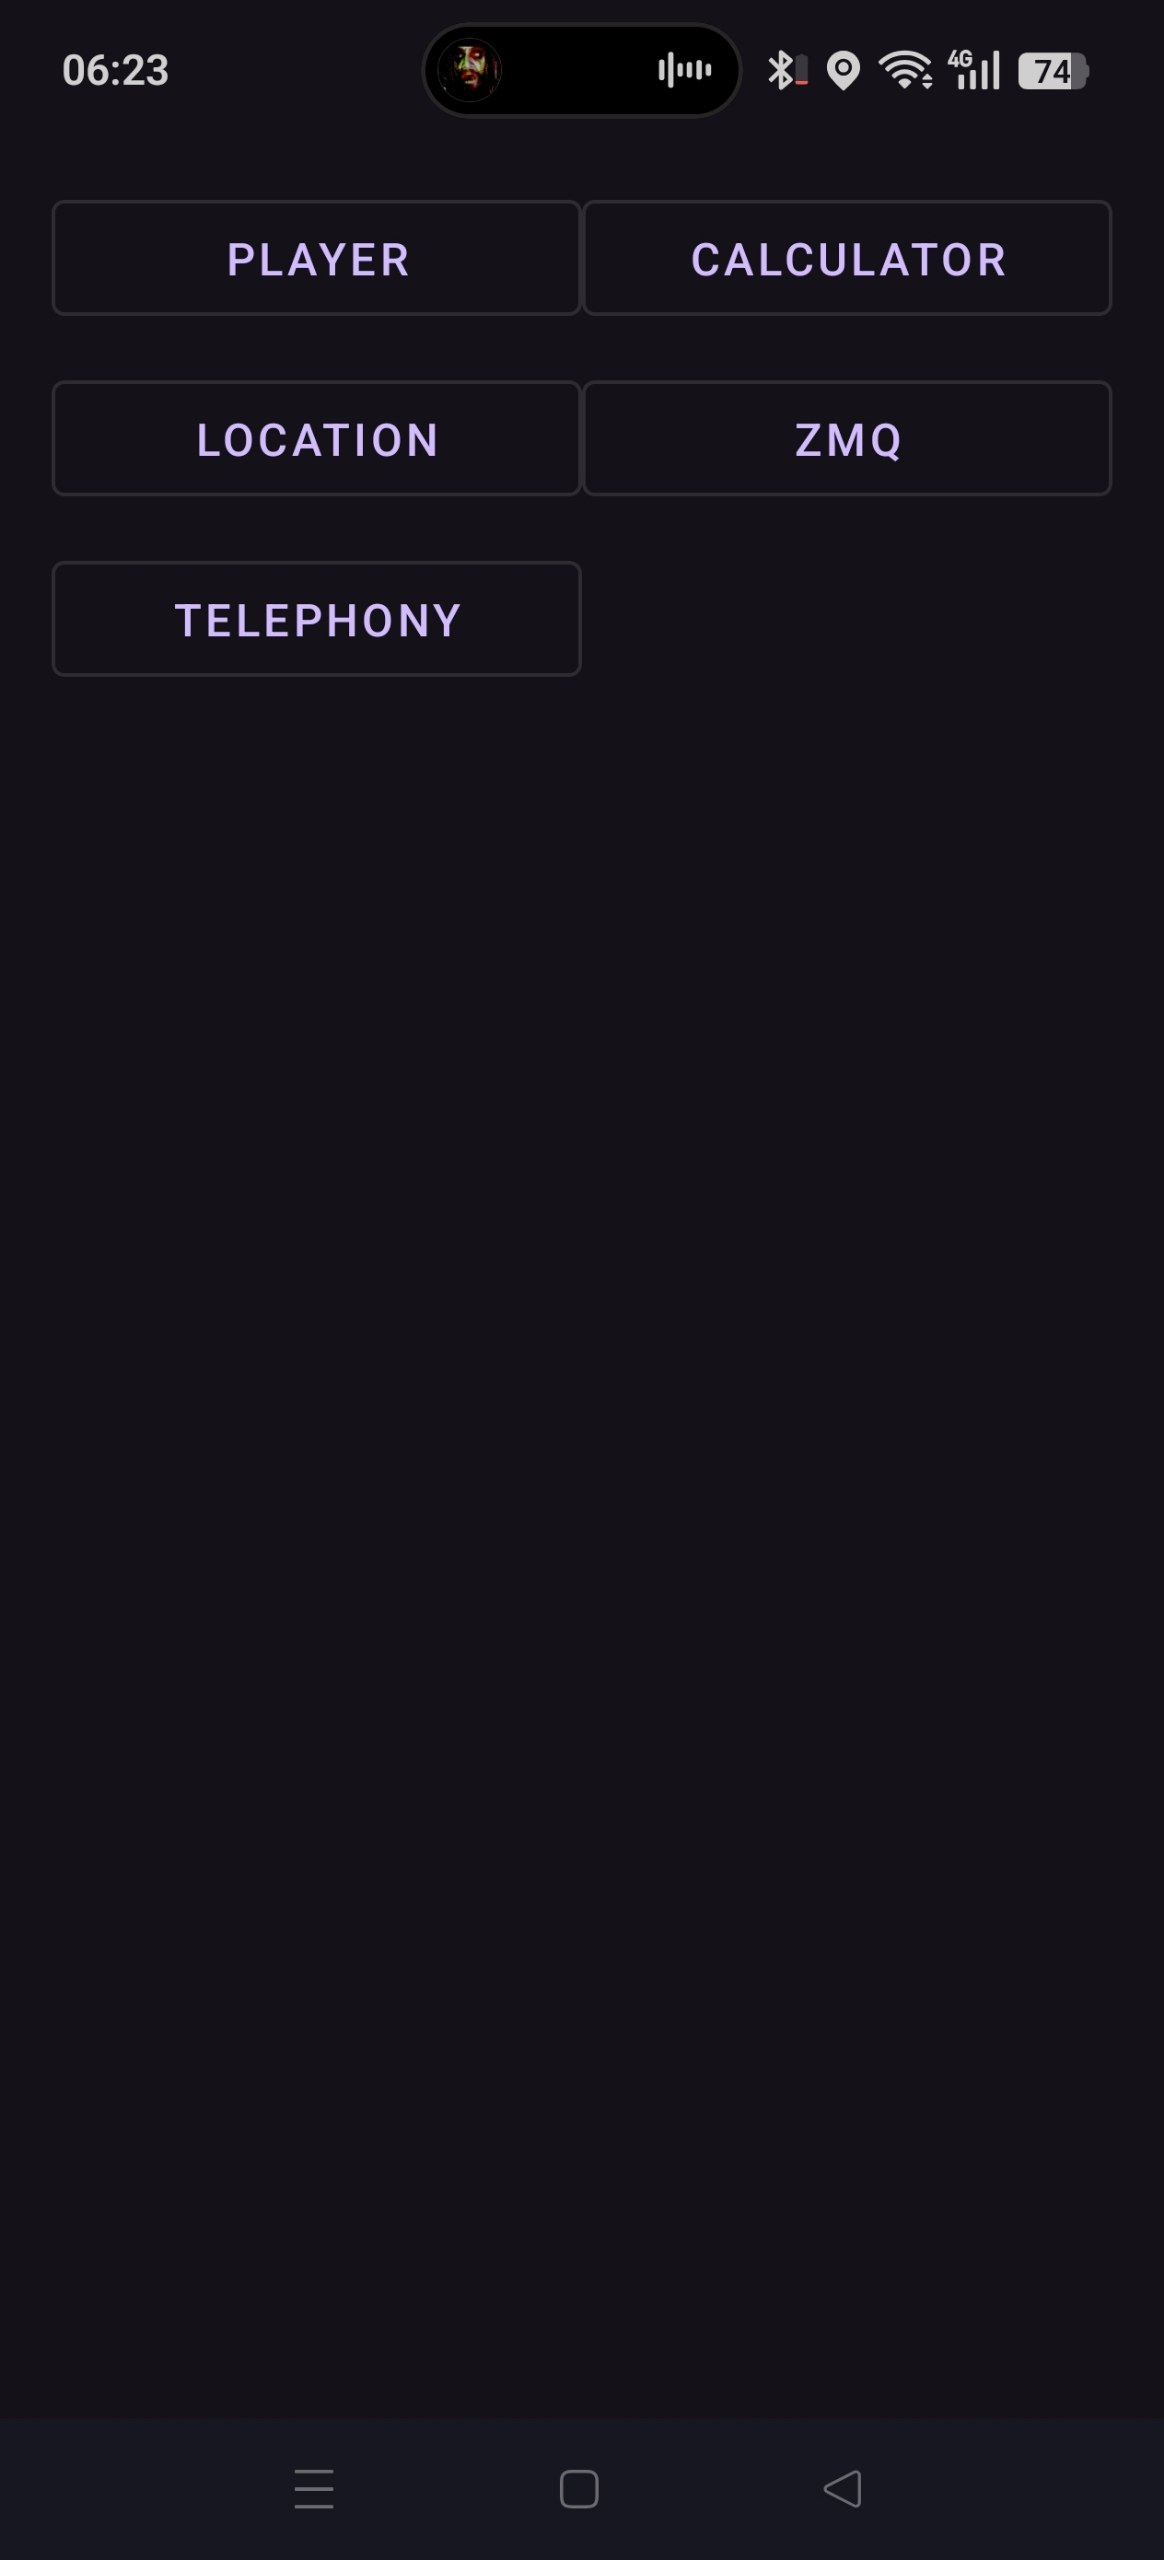
\includegraphics[width=0.7\textwidth,keepaspectratio]{images/android_screen.png}
    \caption{Пример главного экрана Android-приложения}
    \label{fig:android_screen}
\end{figure}

% ------------------- ГЛАВА 2. ТЕОРЕТИЧЕСКАЯ ЧАСТЬ -------------------
\chapter{Теоретическая часть}

\section{Система координат LLA}

\subsection{Широта, долгота, высота}

Для описания положения объекта на Земле используется система LLA,
включающая три параметра.

\textbf{Широта} (Latitude, $\varphi$) --- угол между плоскостью экватора
и вертикалью. Диапазон: $-90^{\circ} \leq \varphi \leq +90^{\circ}$.

\textbf{Долгота} (Longitude, $\lambda$) --- угол от Гринвичского меридиана.
Диапазон: $-180^{\circ} \leq \lambda \leq +180^{\circ}$.

\textbf{Высота} (Altitude, $h$) --- расстояние от эллипсоида WGS-84 до
точки, в метрах.

Пересчёт геодезических координат $(\varphi, \lambda, h)$ в геоцентрические
прямоугольные $(X, Y, Z)$:
\begin{equation}
  X = \bigl(N(\varphi) + h\bigr)\cos\varphi\cos\lambda,
\end{equation}
\begin{equation}
  Y = \bigl(N(\varphi) + h\bigr)\cos\varphi\sin\lambda,
\end{equation}
\begin{equation}
  Z = \bigl(N(\varphi)(1-e^2) + h\bigr)\sin\varphi,
\end{equation}
где $N(\varphi)$ --- радиус кривизны первого вертикала:
\begin{equation}
  N(\varphi) = \frac{a}{\sqrt{1 - e^2\sin^2\varphi}},
\end{equation}
$a = 6\,378\,137$~м (большая полуось WGS-84), $e^2 \approx 0{,}00669438$.

Точность GPS-приёмника смартфона типично 3--10~м.

\subsection{Архитектура сотовых сетей}

\subsubsection{GSM (2G)}

GSM использует TDMA/FDMA. Полоса канала --- 200~кГц, фрейм --- 8 временных
слотов. Основные идентификаторы: MCC, MNC, LAC, CellID, ARFCN, BSIC.

\subsubsection{LTE (4G)}

LTE применяет OFDMA (нисходящий) и SC-FDMA (восходящий). Ключевые
параметры: PCI, TAC, EARFCN, Band.

\subsubsection{NR (5G)}

5G NR поддерживает Sub-6~GHz и mmWave. Идентификаторы: NCI, NRARFCN,
SS-RSRP, SS-RSRQ, SS-SINR.

\subsection{Критерии качества радиосигнала}

\subsubsection{RSSI}

RSSI (Received Signal Strength Indicator) --- суммарная мощность принятого
сигнала:
\begin{equation}
  \mathrm{RSSI} = P_{\mathrm{signal}} + P_{\mathrm{interference}} +
  P_{\mathrm{noise}}, \quad [\text{дБм}].
\end{equation}
Диапазон: от $-113$ до $-51$~дБм.

\subsubsection{RSRP}

RSRP (Reference Signal Received Power) --- мощность опорного сигнала LTE,
усреднённая по ресурсным элементам:
\begin{equation}
  \mathrm{RSRP} = \frac{1}{N_{\mathrm{RE}}} \sum_{k=1}^{N_{\mathrm{RE}}} P_k,
  \quad [\text{дБм}].
\end{equation}
Диапазон: от $-140$ до $-44$~дБм.

\begin{table}[H]
\centering
\caption{Критерии качества LTE-сигнала по RSRP}
\begin{tabular}{lll}
\toprule
\textbf{Уровень} & \textbf{RSRP, дБм} & \textbf{Характеристика}\\
\midrule
Отличный    & $> -80$              & Максимальная скорость\\
Хороший     & от $-80$ до $-90$    & Стабильная передача данных\\
Нормальный  & от $-90$ до $-100$   & Возможны снижения скорости\\
Слабый      & от $-100$ до $-110$  & Частые обрывы соединения\\
Нет сигнала & $< -110$             & Соединение невозможно\\
\bottomrule
\end{tabular}
\end{table}

\subsubsection{RSRQ}

RSRQ (Reference Signal Received Quality) учитывает интерференцию:
\begin{equation}
  \mathrm{RSRQ} = N \cdot \frac{\mathrm{RSRP}}{\mathrm{RSSI}},
  \quad [\text{дБ}],
\end{equation}
где $N$ --- число ресурсных блоков. Диапазон: от $-19{,}5$ до $-3$~дБ.

\subsubsection{SINR}

SINR (Signal-to-Interference-and-Noise Ratio):
\begin{equation}
  \mathrm{SINR} = \frac{P_{\mathrm{signal}}}
                       {P_{\mathrm{interference}} + P_{\mathrm{noise}}},
  \quad [\text{дБ}].
\end{equation}

\subsection{Анализ аномального трафика по правилу 2-сигма}

В \texttt{NetworkTrafficManager} для выявления приложений с необычно высоким
потреблением трафика используется статистический критерий:
\begin{equation}
  \bar{x} = \frac{1}{n}\sum_{i=1}^{n} x_i, \qquad
  \sigma = \sqrt{\frac{1}{n}\sum_{i=1}^{n}(x_i - \bar{x})^2},
\end{equation}
\begin{equation}
  x_{\mathrm{threshold}} = \bar{x} + 2\sigma.
\end{equation}
Приложение считается аномальным, если $x_i > x_{\mathrm{threshold}}$.

\subsection{Клиент-серверный обмен с ZMQ}

ZeroMQ --- высокопроизводительная асинхронная библиотека для обмена
сообщениями. В работе используется паттерн \textbf{PUSH/PULL}:
Android-клиент отправляет JSON-сообщения (PUSH), а C++-сервер получает их
(PULL). Это обеспечивает надёжную доставку без необходимости ручного
управления соединениями.

% ------------------- ГЛАВА 3. ANDROID-ПРИЛОЖЕНИЕ -------------------
\chapter{Android-приложение}

\section{Структура проекта}

Проект \texttt{visprog-feature-geolocator} организован по слоям:
\begin{itemize}
  \item \texttt{data} --- дата-классы:
        \texttt{LocationData}, \texttt{MobileNetworkData},
        \texttt{MobileNetworkDataList};
  \item \texttt{network} --- классы сетевого уровня:
        \texttt{MobileNetworkManager}, \texttt{WebSocketClient},
        \texttt{ApiClient}, \texttt{NetworkTrafficManager},
        \texttt{ZmqManager};
  \item \texttt{services} --- фоновые сервисы:
        \texttt{LocationService}, \texttt{TelephonyService};
  \item \texttt{ui} --- экраны приложения:
        \texttt{MainActivity}, \texttt{TelephonyActivity},
        \texttt{LocationActivity};
  \item \texttt{utils} --- вспомогательные утилиты:
        \texttt{TelephonyDataBus}.
\end{itemize}

\subsection{Получение координат (Практика №6)}

Для работы с GPS требуются разрешения \texttt{ACCESS\_FINE\_LOCATION} и
\texttt{ACCESS\_COARSE\_LOCATION}. Data-класс \texttt{LocationData} хранит
параметры геопозиции и умеет сериализовать себя в JSON:

\begin{lstlisting}[language=Kotlin, caption={data/LocationData.kt}]
data class LocationData(
    val latitude: Double,
    val longitude: Double,
    val altitude: Double,
    val accuracy: Float,
    val time: Long
) {
    fun toJSONObject(): JSONObject {
        return JSONObject().apply {
            put("latitude",  latitude)
            put("longitude", longitude)
            put("altitude",  altitude)
            put("accuracy",  accuracy)
            put("time",      time)
        }
    }
}
\end{lstlisting}

\textbf{Пояснение.} Класс неизменяемый (все поля — \texttt{val}), что
исключает случайное изменение данных после создания объекта. Метод
\texttt{toJSONObject()} преобразует данные в JSON для отправки на сервер.
Поле \texttt{accuracy} хранит радиус ошибки GPS в метрах (типично
3--10~м для современных смартфонов).

\subsection{Данные сотовых сетей (Практика №10)}

\texttt{MobileNetworkManager} обращается к \texttt{TelephonyManager}
через метод \texttt{allCellInfo} и получает параметры всех видимых сот.
Пример обработки LTE:

\begin{lstlisting}[language=Kotlin,
    caption={Обработка LTE-соты в MobileNetworkManager}]
is CellInfoLte -> {
    val id = cellInfo.cellIdentity
    val ss = cellInfo.cellSignalStrength
    networkDataList.add(MobileNetworkData(
        type   = "LTE",
        cellId = id.ci.toString(),
        pci    = validInt(id.pci),
        tac    = validInt(id.tac),
        earfcn = validInt(id.earfcn),
        rsrp   = validInt(ss.rsrp),
        rsrq   = validInt(ss.rsrq),
        rssi   = validInt(ss.rssi)
    ))
}
\end{lstlisting}

\textbf{Пояснение.} Функция \texttt{validInt} заменяет значение
\texttt{Int.MAX\_VALUE} (которое Android возвращает при отсутствии
данных) на $-1$, упрощая дальнейшую обработку на сервере. Аналогичным
образом обрабатываются GSM и NR.

\subsection{Анализ сетевого трафика (Практика №10)}

Реализация правила $2\sigma$ в \texttt{NetworkTrafficManager}:

\begin{lstlisting}[language=Kotlin,
    caption={Фрагмент NetworkTrafficManager.kt}]
val values    = appUsageMap.values.toList()
val mean      = values.average()
val stdDev    = sqrt(
    values.map { (it - mean).pow(2) }.sum() / values.size
)
val threshold = mean + 2 * stdDev
val anomalies = appUsageMap.filter { it.value > threshold }
\end{lstlisting}

\textbf{Пояснение.} Сначала вычисляется среднее значение потребления
трафика по всем приложениям и стандартное отклонение. Порог отсечения
$x_{\mathrm{threshold}} = \bar{x} + 2\sigma$ выбирается так, что при
нормальном распределении за него выходит не более $\approx 2{,}3\%$
значений. Приложения с трафиком выше порога помечаются как аномальные.

\subsection{Фоновый сервис (Практика №11)}

\begin{lstlisting}[language=Kotlin,
    caption={TelephonyService --- отправка данных через ZMQ}]
private fun send() {
    lifecycleScope.launch(Dispatchers.IO) {
        val r = JSONObject()
        if (fGps)
            r.put("location", LocationData(...).toJSONObject())
        val nets = netMgr.getMobileNetworkData().networks
            .filter {
                (it.type == "LTE" && fLte) ||
                (it.type == "NR"  && fNr)
            }
        r.put("mobile_network_data_list", ...)
        push?.send(r.toString())
    }
}
\end{lstlisting}

\textbf{Пояснение.} Сервис работает как \textit{foreground service}:
показывает постоянное уведомление и не выгружается системой. Он создаёт
ZMQ PUSH-сокет и с заданным интервалом отправляет JSON-пакет на сервер.
Фильтры (GPS, LTE, NR) управляются командами, приходящими через второй
PULL-сокет (порт 5559).

\begin{figure}[H]
    \centering
    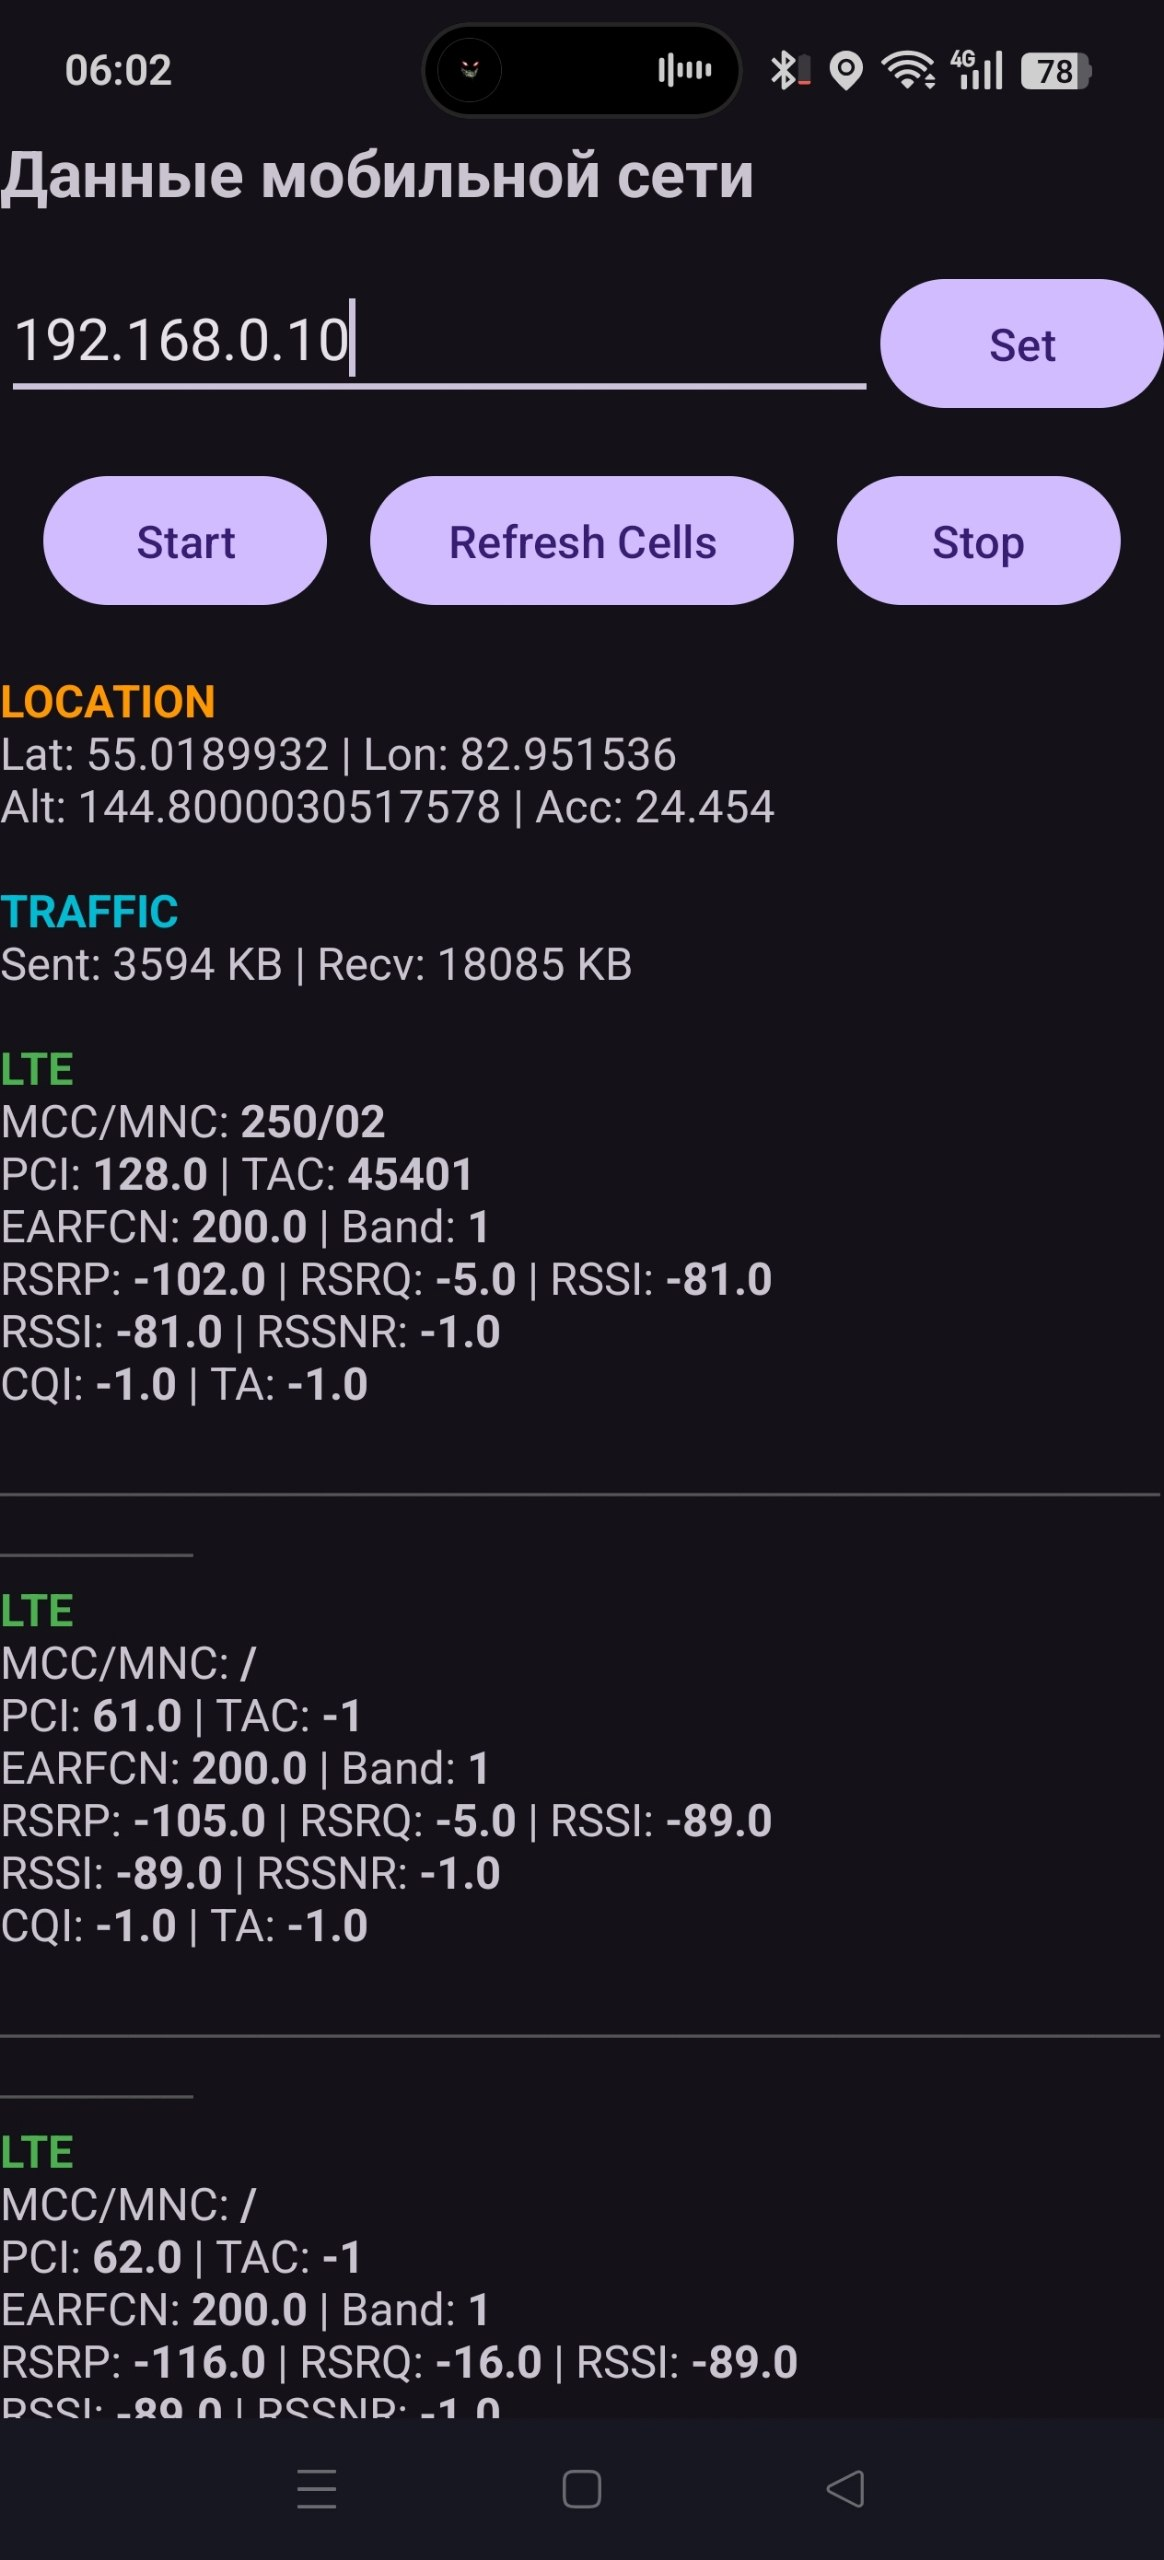
\includegraphics[width=0.6\textwidth,keepaspectratio]{images/telephony_screen.png}
    \caption{Экран телефонии с данными о сотах}
    \label{fig:telephony_screen}
\end{figure}

\section{Диаграмма классов Android}

На рисунке~\ref{fig:android_classes} представлена диаграмма зависимостей
классов Android-приложения (реализована средствами TikZ).

\begin{figure}[H]
\centering
\resizebox{\textwidth}{!}{%
\begin{tikzpicture}[
  font=\small,
  class/.style={
    rectangle, draw, rounded corners=2pt,
    fill=blue!6, minimum width=4.8cm,
    minimum height=0.7cm, align=center,
    text depth=0.3ex
  },
  arrow/.style={-stealth, thick},
  node distance=1.2cm and 2cm
]
% Уровень 1
\node[class] (MA) at (0,0) {MainActivity};
% Уровень 2
\node[class, below left=1.5cm and 1cm of MA] (TA) {TelephonyActivity};
\node[class, below right=1.5cm and 1cm of MA] (LA) {LocationActivity};
% Уровень 3
\node[class, below=of TA] (TS) {TelephonyService};
\node[class, below=of LA] (LS) {LocationService};
% Уровень 4
\node[class, below left=1.2cm and 0.2cm of TS] (MNM) {MobileNetworkManager};
\node[class, below=of TS]                      (NTM) {NetworkTrafficManager};
\node[class, below right=1.2cm and 0.2cm of TS] (WSC) {WebSocketClient};
% Уровень 5
\node[class, below=of MNM] (MND) {MobileNetworkData};
\node[class, below=of NTM] (AC)  {ApiClient};
\node[class, below=of WSC] (LD)  {LocationData};

% Стрелки (минимальное количество)
\draw[arrow] (MA) -- (TA);
\draw[arrow] (MA) -- (LA);
\draw[arrow] (TA) -- (TS);
\draw[arrow] (LA) -- (LS);
\draw[arrow] (TS) -- (MNM);
\draw[arrow] (TS) -- (NTM);
\draw[arrow] (TS) -- (WSC);
\draw[arrow] (MNM) -- (MND);
\draw[arrow] (WSC) -- (AC);
\draw[arrow] (LS)  -- (LD);
\end{tikzpicture}%
}
\caption{Диаграмма классов Android-приложения}
\label{fig:android_classes}
\end{figure}

% ------------------- ГЛАВА 4. BACKEND-СЕРВЕР -------------------
\chapter{Backend-сервер}

\section{Структура проекта C++}

Проект \texttt{rework\_osm\_step14} организован следующим образом:
\begin{itemize}
  \item \texttt{include/} --- заголовочные файлы модулей
        (core, db, net, network, gui);
  \item \texttt{src/} --- исходные файлы реализации;
  \item \texttt{examples/} --- вспомогательные примеры ZMQ на Python.
\end{itemize}

\section{Главный цикл и многопоточность}

\begin{lstlisting}[language=CppSeventeen, caption={src/main.cpp}]
int main() {
    static RuntimeState state;
    std::thread zmq_th(
        RunZmqReceiver, &state, 5558, 5559, true
    );
    if (GuiAppInit(1400, 900, "Backend Control")) {
        while (GuiAppFrame(state)) {}
        GuiAppShutdown();
    }
    state.running = false;
    zmq_th.join();
    return 0;
}
\end{lstlisting}

\textbf{Пояснение.} Приложение запускает два потока. Поток
\texttt{zmq\_th} работает в фоне и принимает данные от Android. Основной
поток выполняет GUI-цикл: \texttt{GuiAppFrame} каждый кадр читает
разделяемое состояние \texttt{RuntimeState} и обновляет интерфейс.
Завершение приложения происходит через флаг \texttt{state.running},
который защищён от гонок за счёт \texttt{std::atomic<bool>}.

\section{ZMQ-приёмник (Практика №7--9)}

\begin{lstlisting}[language=CppSeventeen,
    caption={src/net/zmq\_receiver.cpp (фрагмент)}]
void RunZmqReceiver(
        RuntimeState* st, int dataPort, int cmdPort, bool writeDb) {
    zmq::context_t ctx(1);
    zmq::socket_t  pull(ctx, ZMQ_PULL);
    pull.bind("tcp://0.0.0.0:" + std::to_string(dataPort));
    while (st->running.load()) {
        zmq::message_t msg;
        if (pull.recv(msg, zmq::recv_flags::none)) {
            std::string raw(
                static_cast<char*>(msg.data()), msg.size()
            );
            std::lock_guard<std::mutex> lk(st->mtx);
            ApplyPacket(st, raw, writeDb, db);
            st->packets++;
        }
    }
}
\end{lstlisting}

\textbf{Пояснение.} Сокет \texttt{ZMQ\_PULL} привязывается к порту 5558
и блокируется в ожидании сообщения. При получении пакета берётся мьютекс
(\texttt{lock\_guard}), что предотвращает одновременное чтение данных
GUI-потоком. Затем вызывается \texttt{ApplyPacket} для разбора JSON и
записи в базу данных.

\section{Разбор JSON и обновление состояния}

\begin{lstlisting}[language=CppSeventeen,
    caption={src/core/json\_parser.cpp --- ApplyPacket}]
void ApplyPacket(
        RuntimeState*      st,
        const std::string& raw,
        bool               writeDb,
        PgSqlMinimal&      db) {
    auto j = json::parse(raw);
    ParseLocation(j, st);
    ParseNetworkUsage(j, st);
    for (auto& c : j["mobile_network_data_list"]["MobileNetworks"]) {
        auto n = ParseCell(c);
        st->currentUser.mobileNetworks.push_back(n);
        if (writeDb)
            db.insertRow(MakeDbRow(n, st->currentUser.location));
        AppendSignalPoint(st, n);
        st->heatmapPoints.push_back({
            st->currentUser.location.lat,
            st->currentUser.location.lon,
            static_cast<double>(n.rsrp)
        });
    }
}
\end{lstlisting}

\textbf{Пояснение.} Функция последовательно разбирает три части пакета:
местоположение, статистику трафика и список сот. Для каждой соты точка
добавляется в вектор \texttt{heatmapPoints} (максимум 10\,000 точек ---
старые удаляются). Запись в PostgreSQL выполняется только если флаг
\texttt{writeDb} установлен, что позволяет тестировать сервер без БД.

\section{PostgreSQL (Практика №13)}

\subsection{Схема базы данных}

База данных \texttt{backend\_control} содержит следующие таблицы:
\texttt{user\_equipment}, \texttt{location\_history},
\texttt{telephony\_history}, \texttt{signal\_data},
\texttt{network\_usage\_history}, \texttt{app\_usage\_history},
\texttt{cell\_tower\_cache}.

Основная таблица \texttt{user\_equipment} (одна строка = одно измерение):

\begin{longtable}{|l|l|}
\hline
\textbf{Колонка}    & \textbf{Тип} \\ \hline
\endfirsthead
\hline
\textbf{Колонка}    & \textbf{Тип} \\ \hline
\endhead
imei                & TEXT \\
lat                 & DOUBLE PRECISION \\
lon                 & DOUBLE PRECISION \\
alt                 & DOUBLE PRECISION \\
accuracy            & DOUBLE PRECISION \\
ts                  & BIGINT \\
network\_type       & TEXT \\
mcc                 & TEXT \\
mnc                 & TEXT \\
cell\_id            & TEXT \\
tac                 & TEXT \\
pci                 & INT \\
rsrp                & INT \\
rsrq                & INT \\
rssi                & INT \\
\hline
\caption{Структура таблицы \texttt{user\_equipment}}
\end{longtable}

\begin{figure}[H]
\centering
\resizebox{0.9\textwidth}{!}{%
\begin{tikzpicture}[
  font=\small,
  node distance=1.8cm,
  table/.style={
    rectangle, draw, rounded corners=2pt,
    fill=blue!5, minimum width=4.2cm,
    minimum height=1cm, align=center
  },
  fk/.style={-stealth, dashed, color=red!70!black, thick}
]

\node[table] (ue) {%
  \textbf{user\_equipment}\\[2pt]
  imei, lat, lon, alt,\\
  accuracy, ts,\\
  network\_type, mcc, mnc,\\
  cell\_id, tac, pci,\\
  rsrp, rsrq, rssi%
};

\node[table, below left=1.6cm and 0.6cm of ue] (lh) {%
  \textbf{location\_history}\\[2pt]
  id, latitude,\\
  longitude, altitude,\\
  accuracy, timestamp%
};

\node[table, below right=1.6cm and 0.6cm of ue] (th) {%
  \textbf{telephony\_history}\\[2pt]
  id, cell\_type, pci,\\
  earfcn, rsrp, rsrq,\\
  rssi, timestamp%
};

\node[table, below=1.6cm of lh] (nuh) {%
  \textbf{network\_usage\_history}\\[2pt]
  id, total\_bytes\_sent,\\
  total\_bytes\_received,\\
  timestamp%
};

\node[table, below=1.6cm of th] (auh) {%
  \textbf{app\_usage\_history}\\[2pt]
  id, package\_name,\\
  bytes,\\
  network\_usage\_id,\\
  timestamp%
};

\draw[->, thick] (lh.north) -- (ue.south west);
\draw[->, thick] (th.north) -- (ue.south east);
\draw[fk] (auh.west) to[out=180,in=0]
    node[midway,above,font=\scriptsize]{FK} (nuh.east);
\end{tikzpicture}%
}
\caption{Схема базы данных \texttt{backend\_control}}
\label{fig:db_schema}
\end{figure}

Единственная явная внешняя связь:
\texttt{app\_usage\_history.network\_usage\_id}~$\rightarrow$
\texttt{network\_usage\_history.id}. Остальные таблицы логически связаны
через временны́е метки.

\subsection{Код для работы с БД}

\begin{lstlisting}[language=CppSeventeen,
    caption={src/db/pgsql\_minimal.cpp --- вставка строки}]
bool PgSqlMinimal::insertRow(const DbSignalRow& x) {
    const char* vals[] = {
        x.imei.c_str(), x.lat.c_str(), x.lon.c_str(),
        x.alt.c_str(),  x.acc.c_str(), x.ts.c_str(),
        /* ... остальные 15 полей ... */
    };
    const char* q =
        "INSERT INTO user_equipment"
        "(imei,lat,lon,alt,accuracy,ts,"
        " network_type,mcc,mnc,cell_id,tac,"
        " pci,rsrp,rsrq,rssi)"
        " VALUES($1,$2,$3,$4,$5,$6,"
        "        $7,$8,$9,$10,$11,"
        "        $12,$13,$14,$15)";
    PGresult* r = PQexecParams(
        conn_, q, 15, nullptr, vals, nullptr, nullptr, 0
    );
    bool ok = r && PQresultStatus(r) == PGRES_COMMAND_OK;
    PQclear(r);
    return ok;
}
\end{lstlisting}

\textbf{Пояснение.} Использование параметризованного запроса
(\texttt{\$1}, \texttt{\$2}, …) вместо конкатенации строк защищает от
SQL-инъекций. Функция \texttt{PQexecParams} передаёт параметры отдельно
от тела запроса; сервер PostgreSQL компилирует план один раз и
переиспользует его.

\section{GUI на ImGui (Практика №9)}

\begin{lstlisting}[language=CppSeventeen,
    caption={src/gui\_app.cpp --- отрисовка вкладок}]
if (ImGui::BeginTabBar("tabs")) {
    if (ImGui::BeginTabItem("Главная"))
        { TabMain(state);     ImGui::EndTabItem(); }
    if (ImGui::BeginTabItem("Графики"))
        { TabSignals(state);  ImGui::EndTabItem(); }
    if (ImGui::BeginTabItem("Локальные"))
        { TabLocal(state);    ImGui::EndTabItem(); }
    if (ImGui::BeginTabItem("Карта"))
        { TabMap(state);      ImGui::EndTabItem(); }
    if (ImGui::BeginTabItem("Телефония"))
        { TabTelephony(state);ImGui::EndTabItem(); }
    if (ImGui::BeginTabItem("Фильтры"))
        { TabFilters(state);  ImGui::EndTabItem(); }
    ImGui::EndTabBar();
}
\end{lstlisting}

\textbf{Пояснение.} ImGui работает в режиме «немедленного» рендеринга
(\textit{immediate mode}): каждый кадр UI полностью перестраивается.
Вкладки позволяют разбить интерфейс на логические разделы: главная
страница со статусом подключения, графики временны́х рядов RSRP/RSRQ,
список локальных данных, карта OSM, таблица сот и панель управления
фильтрами.

\begin{figure}[H]
    \centering
    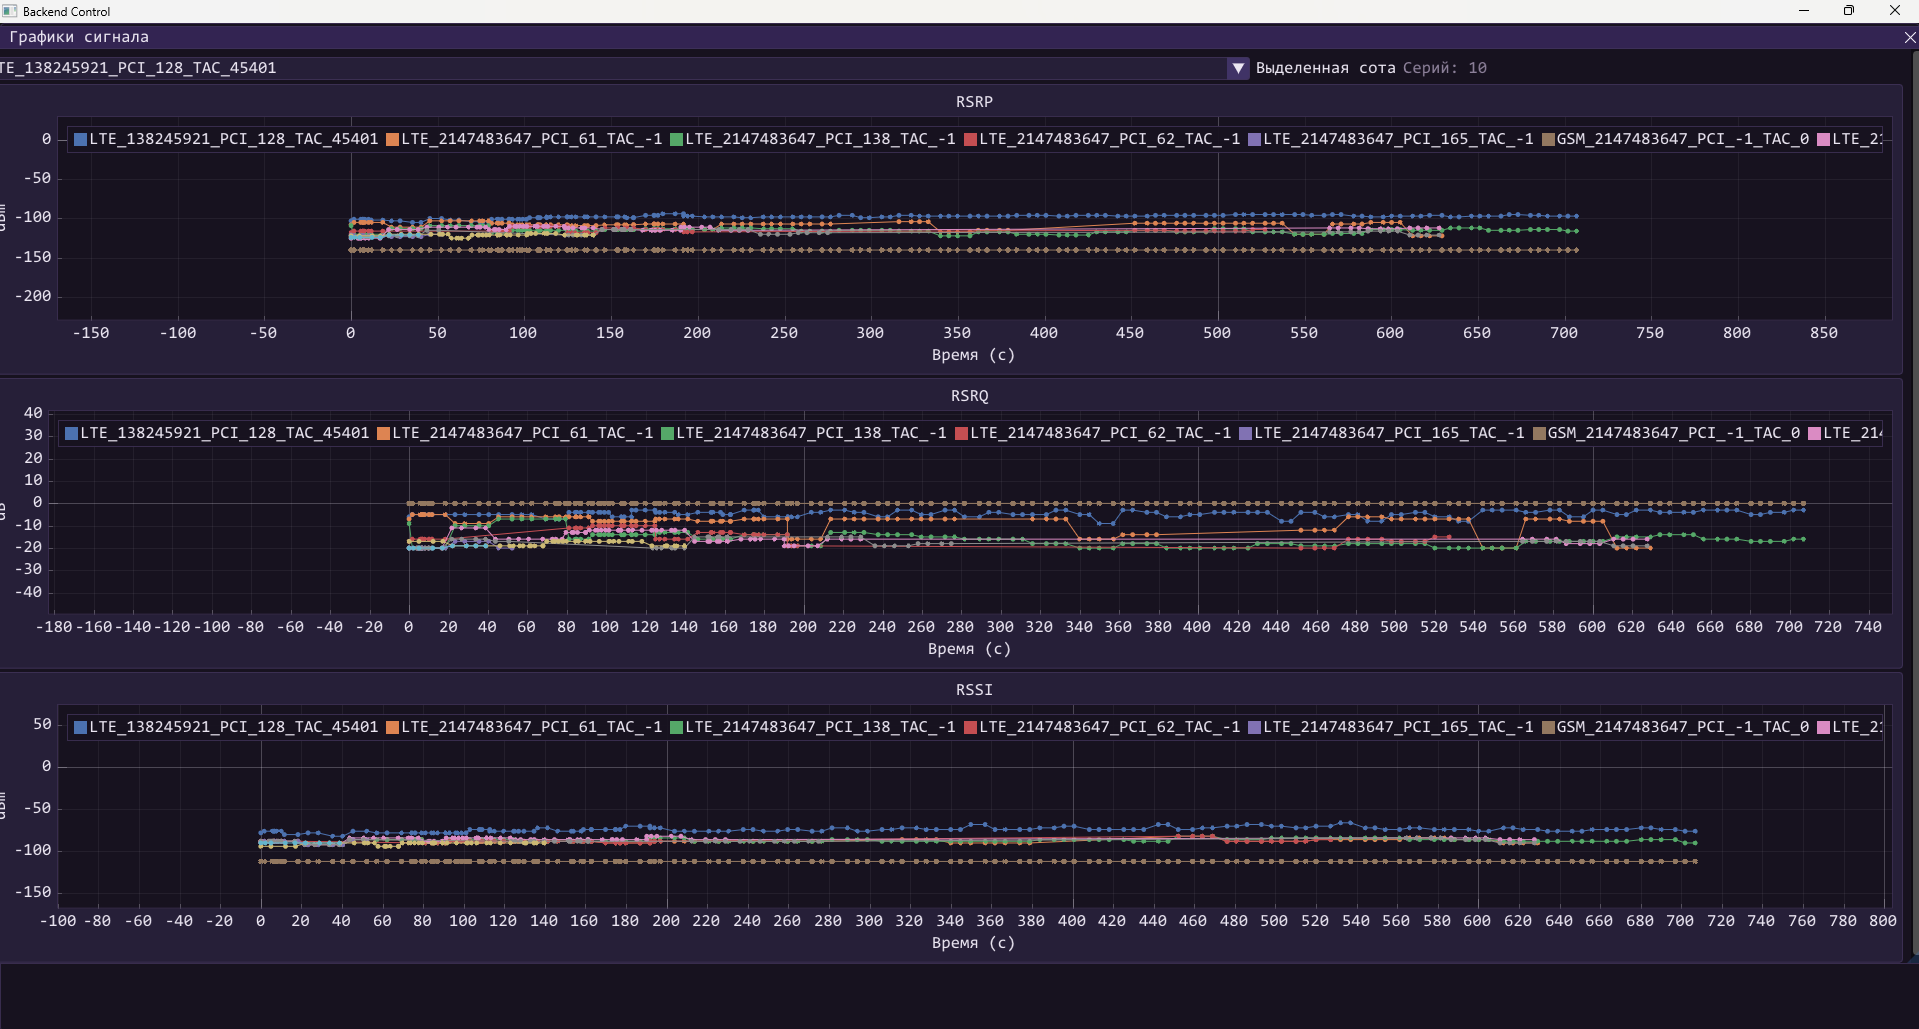
\includegraphics[width=0.8\textwidth,keepaspectratio]{images/backend_gui.png}
    \caption{Интерфейс серверной части (ImGui)}
    \label{fig:gui_screenshot}
\end{figure}

\section{Карта OpenStreetMap и проекция Меркатора (Практика №14)}

\subsection{Преобразование координат в тайлы}

OpenStreetMap использует проекцию Web Mercator (EPSG:3857).
Преобразование широты и долготы в индексы тайлов:
\begin{equation}
X_{\text{merc}} = \lambda_{\text{WGS84}}, \quad
Y_{\text{merc}} = \ln\!\left(\tan\varphi_{\text{WGS84}} +
                  \frac{1}{\cos\varphi_{\text{WGS84}}}\right),
\end{equation}
\begin{equation}
x_{\text{norm}} = 0{,}5 + \frac{X_{\text{merc}}}{360},\quad
y_{\text{norm}} = 0{,}5 - \frac{Y_{\text{merc}}}{2\pi},
\end{equation}
\begin{equation}
x_{\text{tile}} = \bigl\lfloor 2^{\text{zoom}} \cdot x_{\text{norm}}
                  \bigr\rfloor,\quad
y_{\text{tile}} = \bigl\lfloor 2^{\text{zoom}} \cdot y_{\text{norm}}
                  \bigr\rfloor.
\end{equation}

Пример для \texttt{lat=55.007969}, \texttt{lon=82.944546},
\texttt{zoom=16}:
\begin{itemize}
  \item $X_{\text{merc}}=82{,}944546$, $Y_{\text{merc}}=1{,}154477$;
  \item $x_{\text{norm}}=0{,}7304015$, $y_{\text{norm}}=0{,}3162593$;
  \item $2^{16}=65536$, $x_{\text{tile}}=47867$, $y_{\text{tile}}=20726$.
\end{itemize}

Реализация в \texttt{osm\_math.h}:

\begin{lstlisting}[language=CppSeventeen,
    caption={include/osm\_math.h --- основные функции}]
inline double TileXExact(double lon, int zoom) {
    return (1 << zoom) * (0.5 + lon / 360.0);
}
inline double TileYExact(double lat, int zoom) {
    double latRad = lat * M_PI / 180.0;
    double mercY  = log(tan(latRad) + 1.0 / cos(latRad));
    return (1 << zoom) * (0.5 - mercY / (2.0 * M_PI));
}
\end{lstlisting}

\textbf{Пояснение.} Тайлы загружаются асинхронно через cURL в пуле
потоков, кэшируются на диске в виде PNG-файлов и отображаются через
\texttt{ImPlot::PlotImage}. Такой подход позволяет работать оффлайн после
первого прохода по маршруту.

\begin{figure}[H]
    \centering
    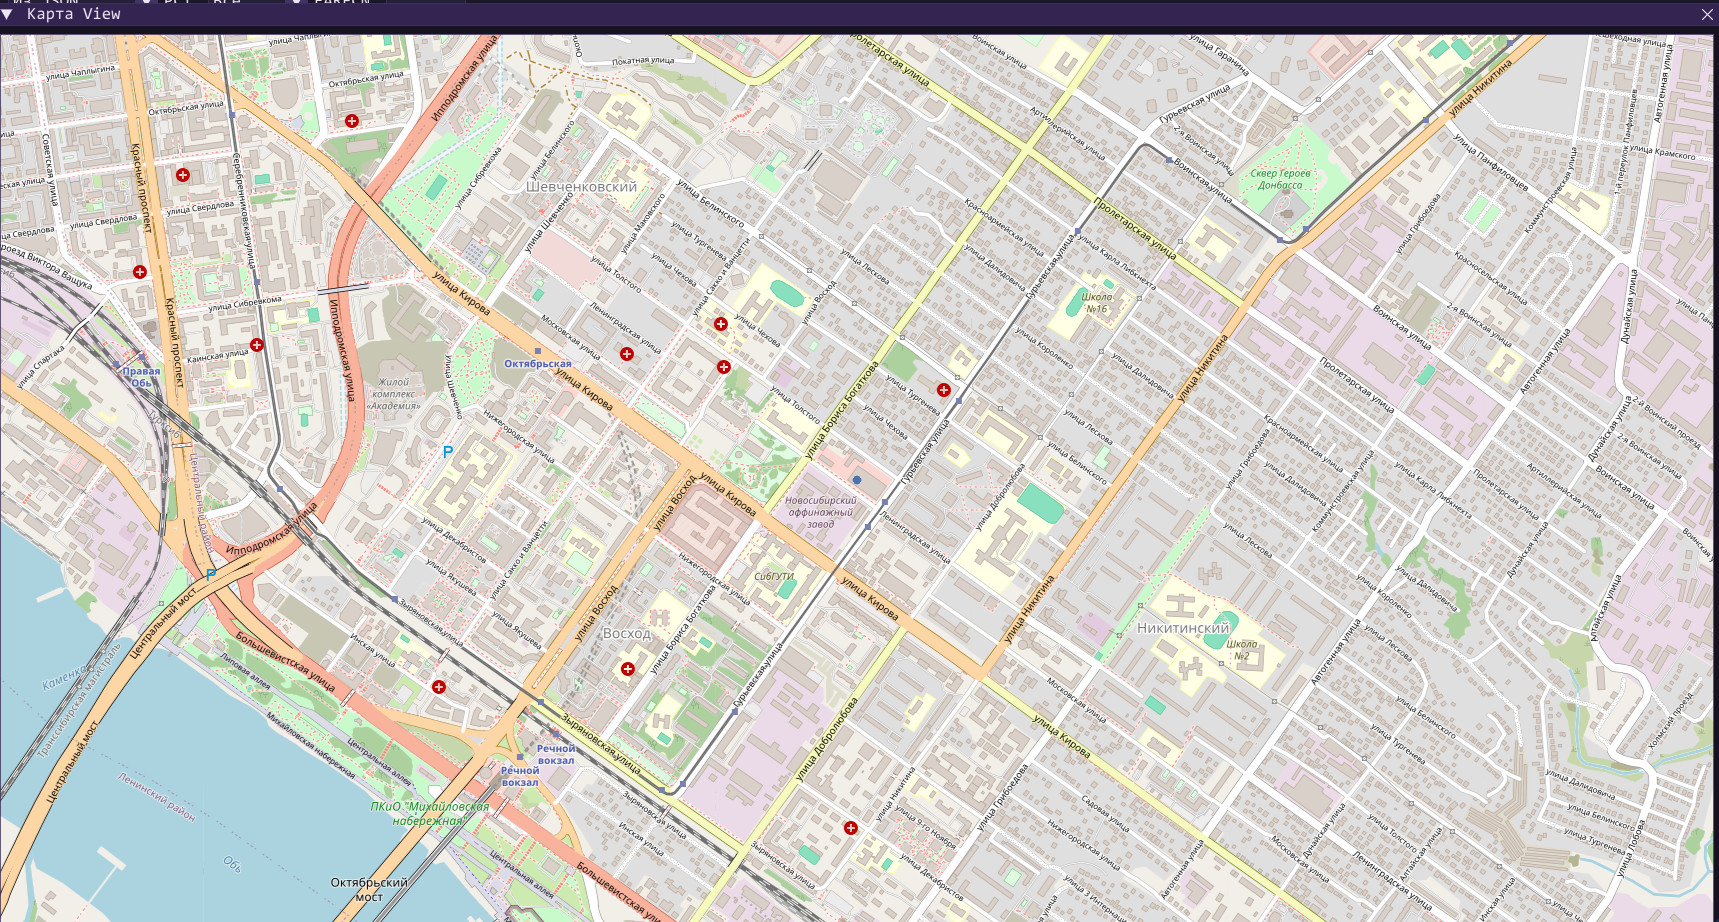
\includegraphics[width=0.7\textwidth,keepaspectratio]{images/osm_map.png}
    \caption{Отображение тайлов OpenStreetMap в GUI}
    \label{fig:osm_screenshot}
\end{figure}

\section{Тепловая карта методом IDW (Практика №15)}

\subsection{Алгоритм IDW}

Интерполяция обратно взвешенных расстояний (Inverse Distance Weighting):
\begin{equation}
  \mathrm{value}(x) =
  \begin{cases}
    \dfrac{\displaystyle\sum_{i=1}^{N} w_i(x)\cdot \mathrm{value}_i}
          {\displaystyle\sum_{i=1}^{N} w_i(x)}, & d(x,x_i) \neq 0,\\[12pt]
    \mathrm{value}_i, & d(x,x_i) = 0,
  \end{cases}
\end{equation}
где весовая функция:
\begin{equation}
  w_i(x) = \frac{1}{d(x,x_i)^p}.
\end{equation}
В реализации $p=2$ (квадрат расстояния), радиус поиска
$R \in [10, 40]$~метров.

Расстояние между двумя точками на сфере вычисляется по формуле
гаверсинуса:
\begin{equation}
  \begin{aligned}
  a &= \sin^2\frac{\Delta\varphi}{2} +
       \cos\varphi_1 \cos\varphi_2 \sin^2\frac{\Delta\lambda}{2},\\
  d &= 2R_{\oplus} \cdot \operatorname{atan2}(\sqrt{a},\,\sqrt{1-a}),
  \end{aligned}
\end{equation}
где $R_{\oplus}=6\,371\,000$~м --- средний радиус Земли.

\subsection{Фрагмент реализации}

\begin{lstlisting}[language=CppSeventeen,
    caption={src/core/heatmap\_generator.cpp --- IDW}]
for (const auto& pt : pts) {
    int x0 = static_cast<int>(
        (pt.lon - dLon - minLon) / (maxLon - minLon) * W) - 1;
    int x1 = static_cast<int>(
        (pt.lon + dLon - minLon) / (maxLon - minLon) * W) + 1;
    for (int py = y0; py <= y1; ++py)
    for (int px = x0; px <= x1; ++px) {
        double d = haversine(p_lat, p_lon, pt.lat, pt.lon);
        if (d > 0.0 && d <= radius) {
            double w      = 1.0 / std::pow(d, power);
            sumW[idx]    += w;
            sumV[idx]    += w * pt.value;
        } else if (d == 0.0) {
            sumW[idx]     = 1.0;
            sumV[idx]     = pt.value;
        }
    }
}
\end{lstlisting}

\textbf{Пояснение.} Для ускорения расчётов каждая точка влияет только
на пиксели в пределах прямоугольника, соответствующего радиусу $R$ в
географических координатах. Это снижает сложность с $O(NW\!H)$ до
$O(N \cdot r^2)$, где $r$ --- радиус в пикселях. Итоговая текстура
накладывается на карту через \texttt{ImPlot::PlotImage} с альфа-каналом.

\subsection{Цветовое кодирование RSRP (согласно коду)}

\begin{table}[H]
\centering
\caption{Цветовая схема тепловой карты (из heatmap\_generator.cpp)}
\label{tab:heatmap_colors}
\begin{tabular}{lll}
\toprule
\textbf{Уровень} & \textbf{RSRP, дБм} & \textbf{Цвет (RGB, Alpha)} \\
\midrule
Отличный         & $> -85$              & Красный (255, 0, 0, 255) \\
Хороший          & $-85 \ldots -95$     & Оранжевый (255, 165, 0, 255) \\
Нормальный       & $-95 \ldots -105$    & Голубой (0, 255, 255, 255) \\
Слабый           & $-105 \ldots -120$   & Тёмно-синий (0, 0, 139, 255) \\
Нет сигнала      & $< -120$             & Серый (60, 60, 60, 180) \\
\bottomrule
\end{tabular}
\end{table}

\begin{figure}[H]
    \centering
    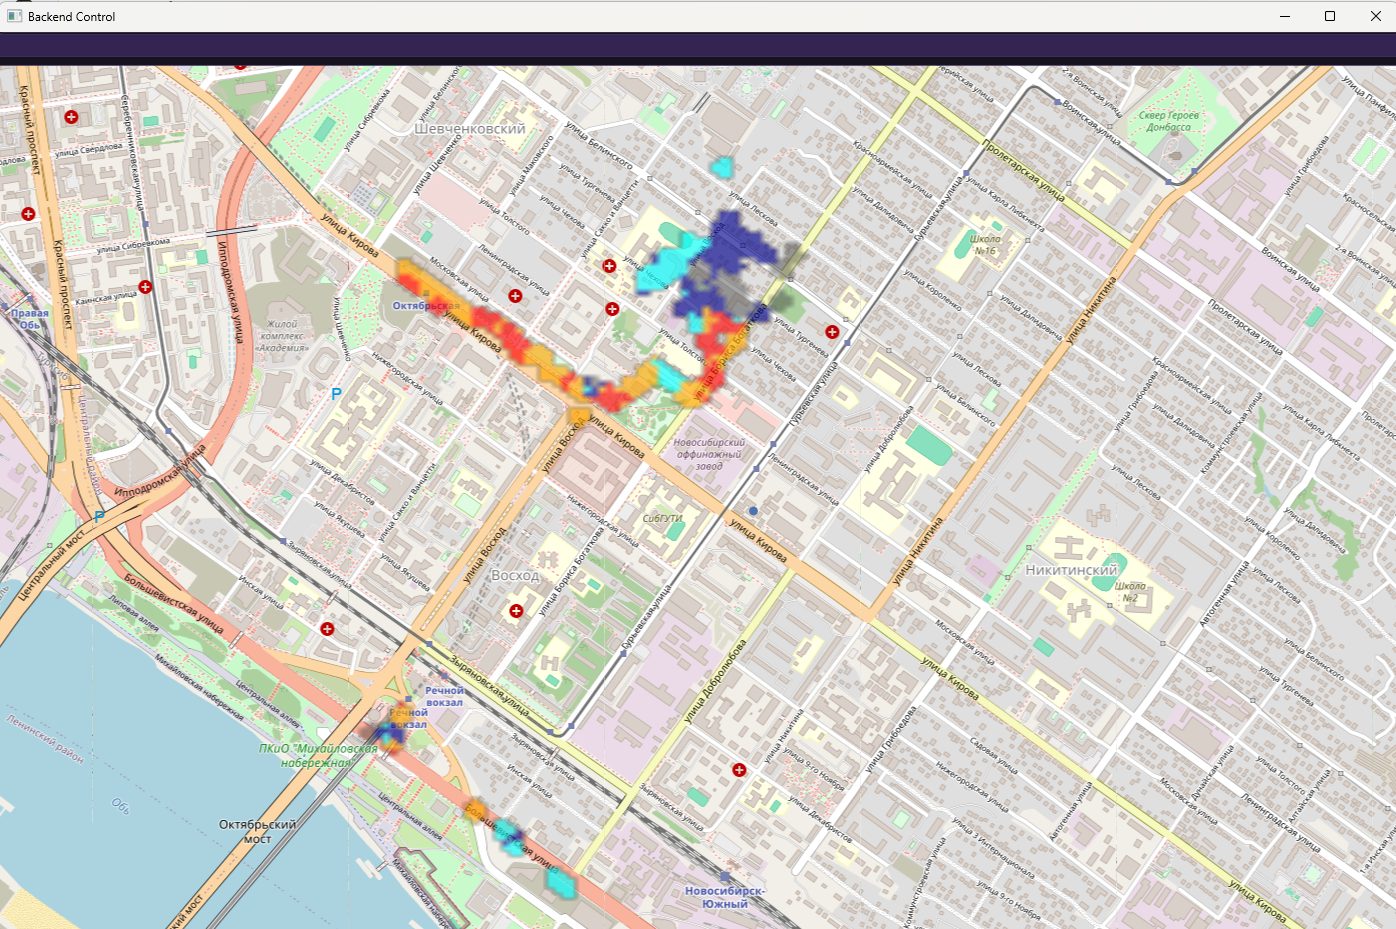
\includegraphics[width=0.7\textwidth,keepaspectratio]{images/heatmap.png}
    \caption{Тепловая карта уровня сигнала RSRP}
    \label{fig:heatmap_screenshot}
\end{figure}

% ------------------- ГЛАВА 5. ОБЩАЯ АРХИТЕКТУРА ПАК -------------------
\chapter{Общая архитектура ПАК}

\section{Структурная схема}

На рисунке~\ref{fig:arch} представлена полная архитектура ПАК, выполненная
в виде графического файла.

\begin{figure}[H]
    \centering
    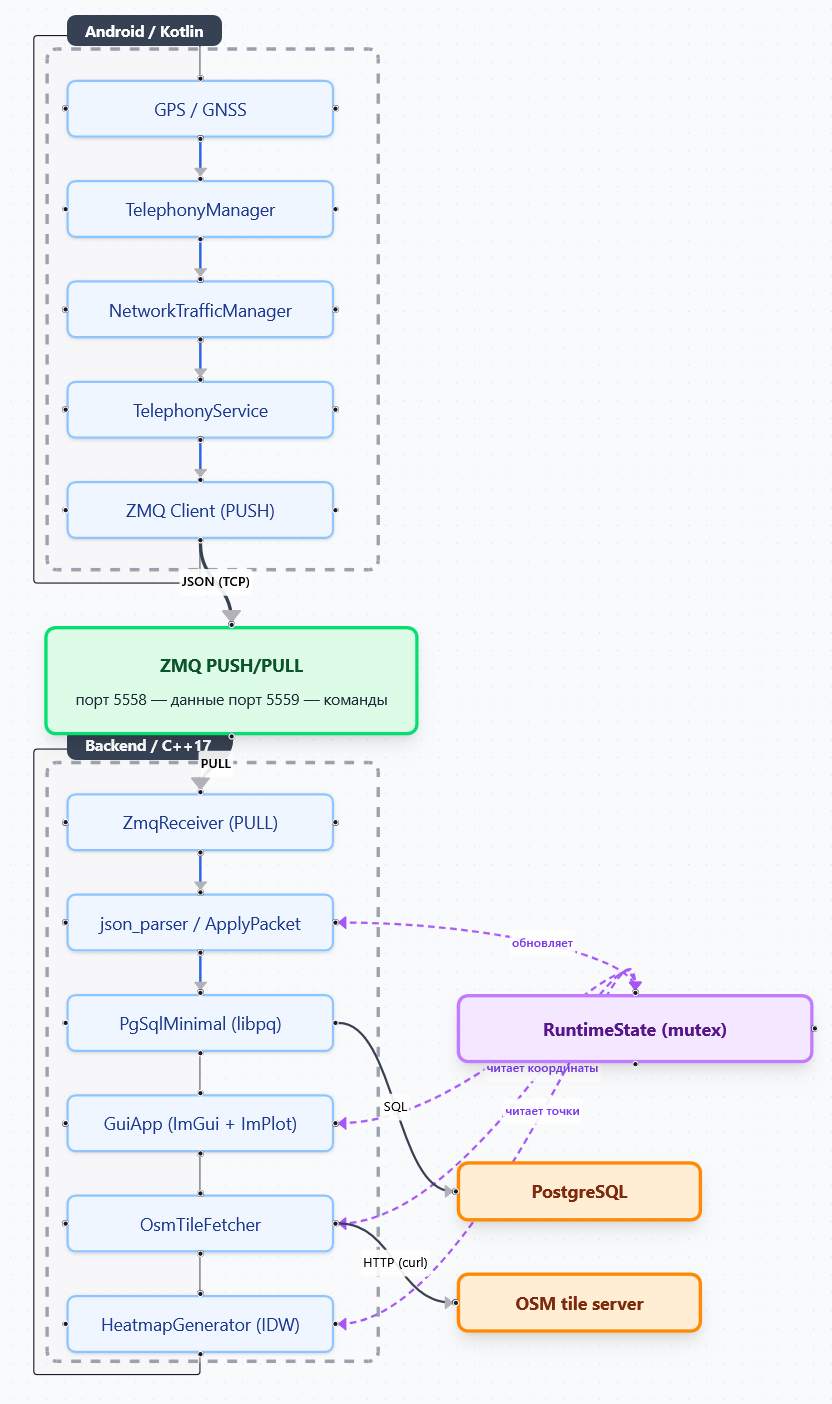
\includegraphics[width=\textwidth,keepaspectratio]{images/architecture.png}
    \caption{Архитектура ПАК}
    \label{fig:arch}
\end{figure}

\section{Поток данных}

\begin{enumerate}
  \item \texttt{TelephonyService} собирает GPS-координаты, параметры
        сотовых сетей и статистику трафика.
  \item Сформированный JSON-пакет отправляется через ZMQ PUSH на порт 5558.
  \item \texttt{RunZmqReceiver} (PULL) принимает пакет и вызывает
        \texttt{ApplyPacket}.
  \item \texttt{ApplyPacket} разбирает JSON, обновляет
        \texttt{RuntimeState} (под мьютексом) и вставляет запись в
        PostgreSQL.
  \item GUI-поток читает \texttt{RuntimeState} и обновляет графики,
        таблицы и статус-панель.
  \item \texttt{OsmTileFetcher} асинхронно загружает тайлы карты;
        \texttt{HeatmapGenerator} строит тепловую карту методом IDW
        по накопленным точкам.
\end{enumerate}

% ------------------- ЗАКЛЮЧЕНИЕ -------------------
\chapter{Заключение}

В ходе выполнения практических работ №~6--15 был спроектирован и
реализован программно-аппаратный комплекс для мониторинга качества
мобильной связи. Получены следующие практические навыки:

\begin{itemize}
  \item разработка Android-приложений на Kotlin: Location~API,
        TelephonyManager, Foreground~Service;
  \item клиент-серверные системы на ZeroMQ:
        паттерны REQ/REP и PUSH/PULL;
  \item многопоточность C++17:
        \texttt{std::thread}, \texttt{std::mutex}, \texttt{std::atomic};
  \item работа с PostgreSQL из C++ через библиотеку \texttt{libpq};
  \item GUI Dear ImGui + ImPlot:
        вкладки, графики, обновление в реальном времени;
  \item система тайлов OpenStreetMap,
        проекция Меркатора, декодирование PNG через cURL;
  \item пространственная интерполяция IDW с радиусным ограничением;
  \item рефакторинг кода по модулям (ZMQ, DB, GUI, OSM, Heatmap);
  \item система контроля версий Git:
        ветки, merge request, submodule.
\end{itemize}

Созданный ПАК позволяет проводить полноценные драйв-тесты и визуализировать
покрытие мобильной сети на интерактивной карте. Разработанный код является
модульным и может быть расширен для поддержки новых технологий (например,
5G~NR standalone) и дополнительных источников данных.

% ------------------- СПИСОК ЛИТЕРАТУРЫ -------------------
\nocite{*}
\printbibliography[title=Список использованных источников]

\end{document}